\begin{figure}
        \centering
        \begin{subfigure}[b]{0.9\textwidth}
                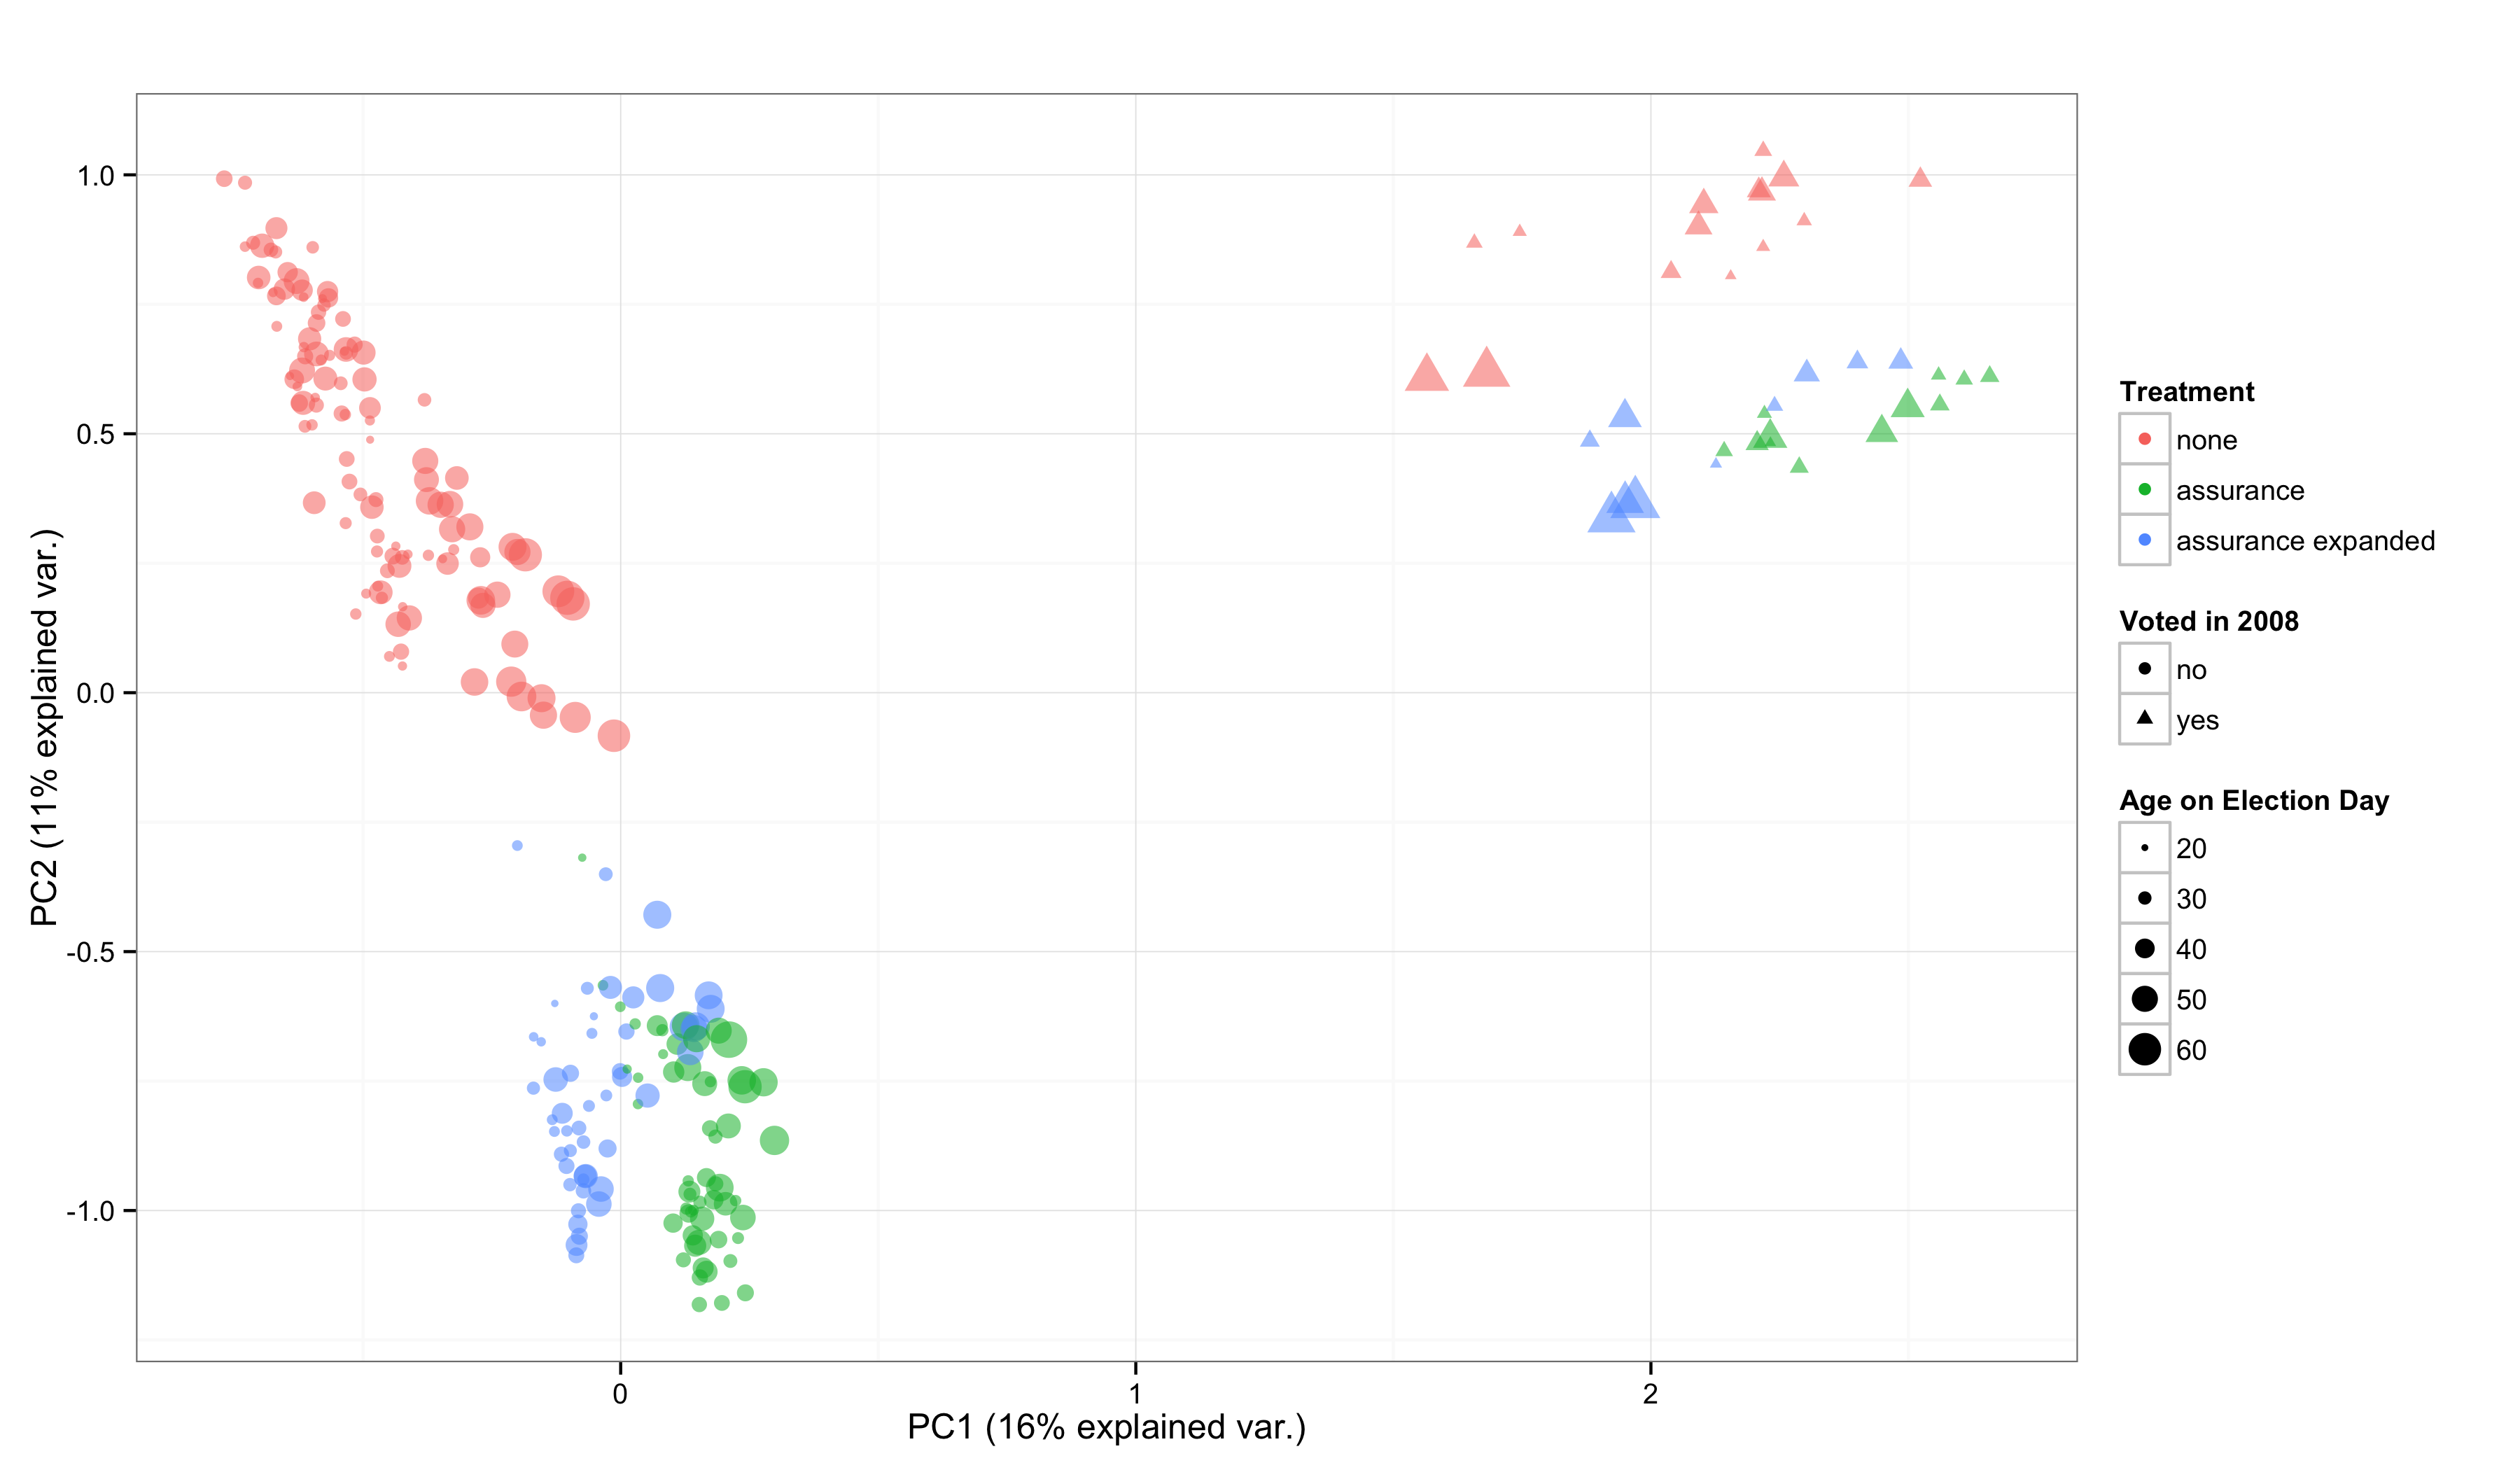
\includegraphics[width=\textwidth]{figures/prox_cond_vote_top.png}
                \caption{Proximity plot with overlaid explanatory variables.}
                \label{fig:prox_top}
        \end{subfigure}%
        ~ %add desired spacing between images, e. g. ~, \quad, \qquad, \hfill etc.
          %(or a blank line to force the subfigure onto a new line)

        \begin{subfigure}[b]{0.9\textwidth}
                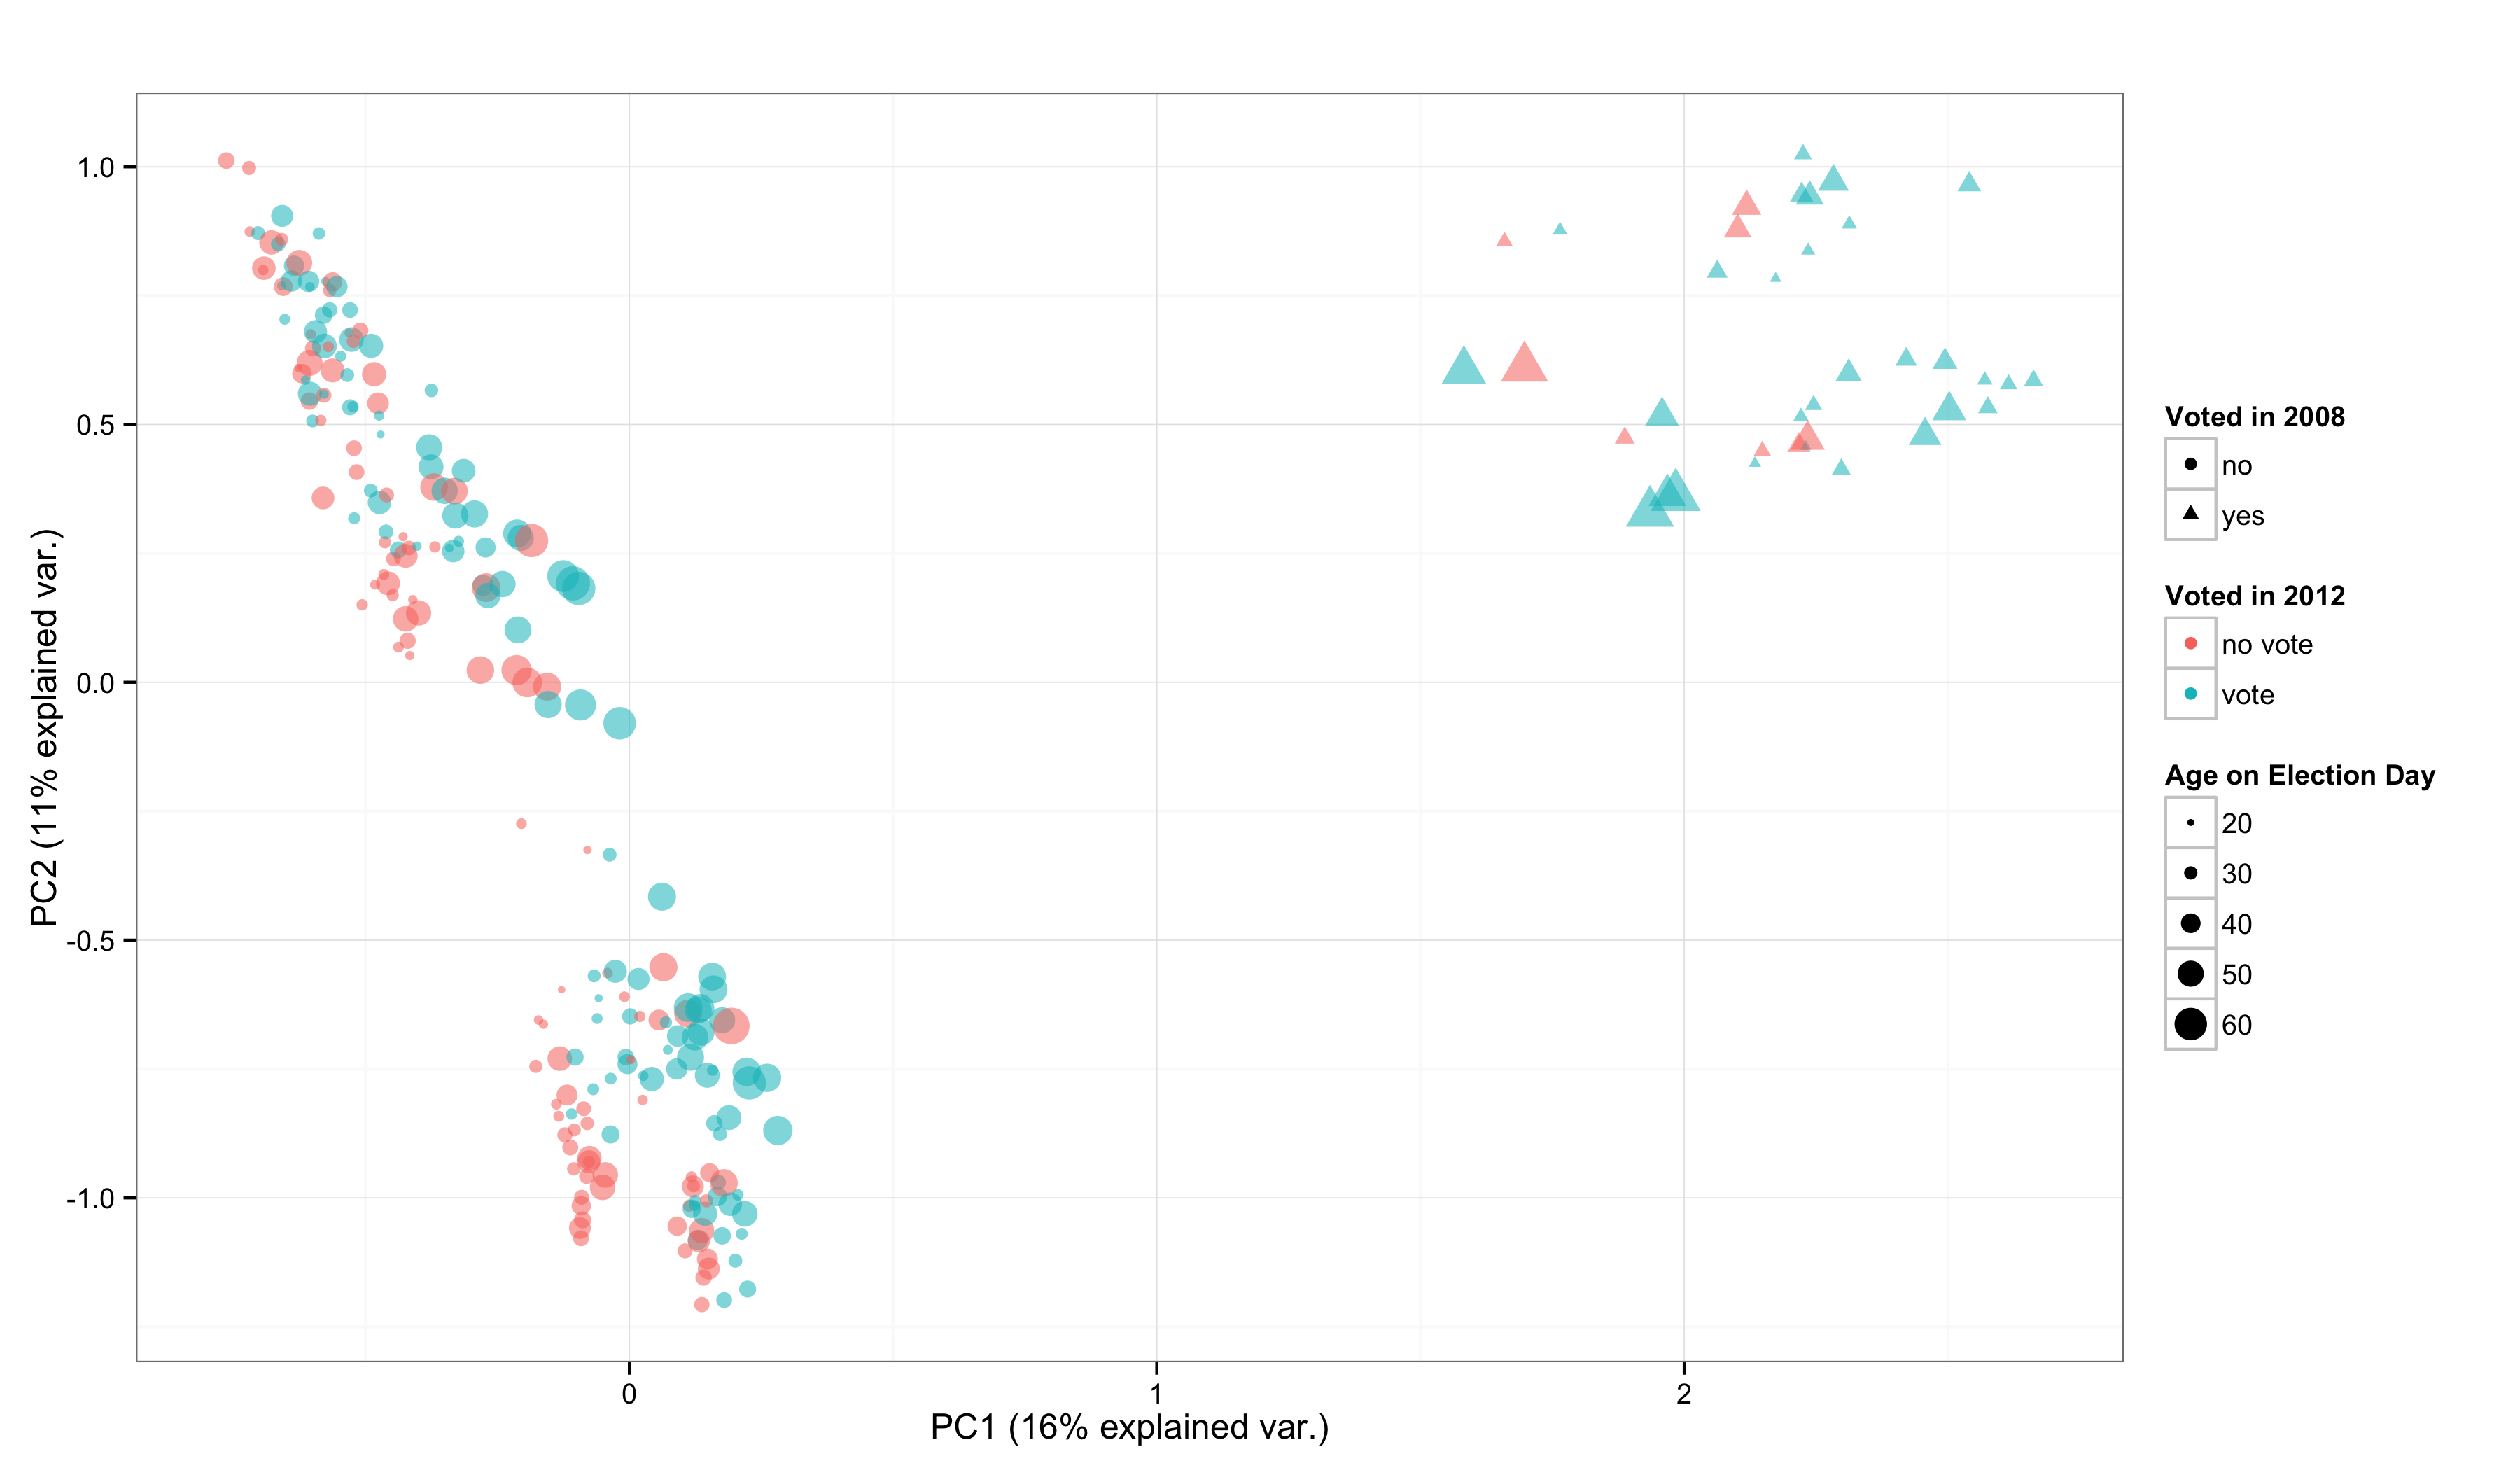
\includegraphics[width=\textwidth]{figures/prox_cond_vote_bottom.png}
                \caption{Proximity plot with overlaid explanatory variables.}
                \label{fig:prox_bottom}
        \end{subfigure}
        \caption{The first two components of PCA of the proximity matrix of a Random Forest fit to ex-felons that have registered to vote, which shows the latent similarity of observations in the space spanned by the predictors.}
        \label{fig:prox}
\end{figure}
